
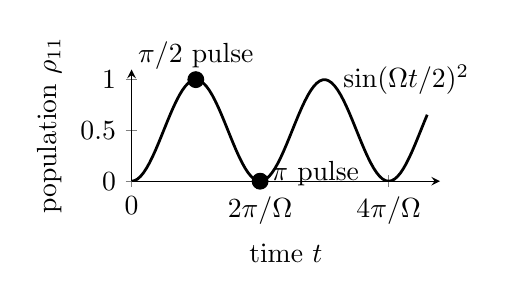
\begin{tikzpicture}


\begin{axis}[no markers, 
        domain=0:2.3, ymin=0, ymax=1.1, xmax =2.4,
        axis lines = left, height=3cm,
           width= 5.5cm,ylabel={population $\rho_{11}$},xlabel=time $t$,           xticklabels = {0, $2 \pi / \Omega$, $4 \pi / \Omega$}, xtick = {0,1,2}           
           ]
\addplot [line width=1pt,samples=100]    {(sin(180* x)^2};

\coordinate (p) at (0.5,1);
    \coordinate (p2) at (1,0);
           \coordinate (ls) at (1.5,1);

       
\end{axis}

\draw[fill] (p) circle (1mm);
\node[above] at (p) {$\pi/2$ pulse};
    
\draw[fill] (p2) circle (1mm);
\node[xshift=7mm, yshift=1mm] at (p2) {$\pi$ pulse};
\node[right] at (ls) {\ $\sin (\Omega t / 2)^2$};

\end{tikzpicture}

